\label{fs-framework}

Our task is to design a framework for end-to-end text streams multi-classification that overcomes the challenges mentioned above. We assume that there are two types of input streams: pre-labeled and raw. Elements from raw stream must be labeled by a classifier and delivered to end-user. The pre-labeled stream is used for updating a machine learning model with new data.

\begin{figure}[htbp]
  \centering
  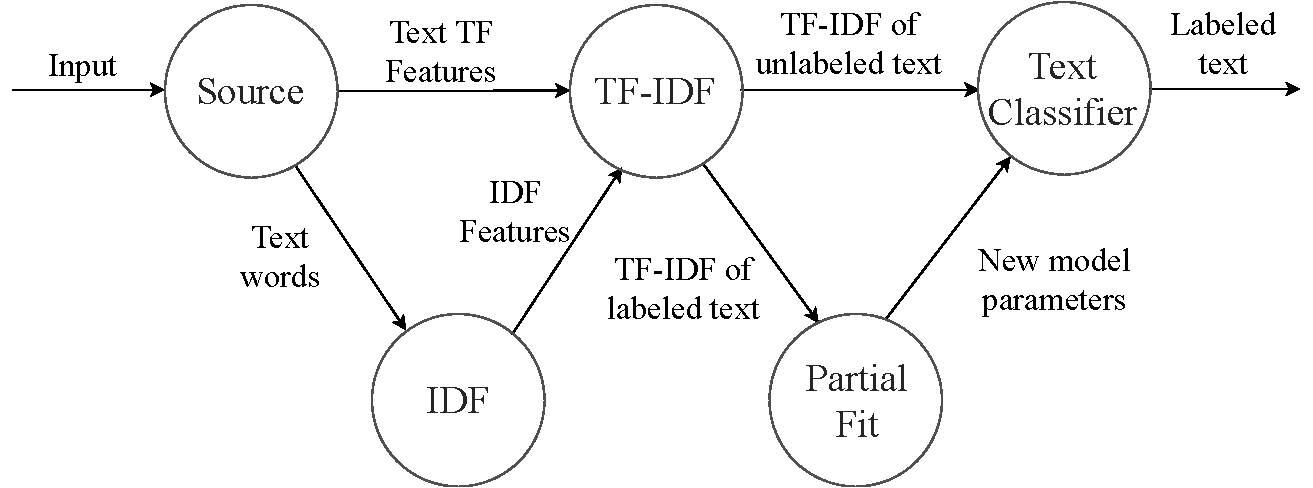
\includegraphics[scale=0.48]{pics/logical-graph}
  \caption{The logical graph}
  \label {logical_graph}
\end{figure}

\subsection{Data flow \label{DF}}

\subsubsection{Predicting pipeline}

Typical texts classification pipeline consists of two steps. The first one is computing TF-IDF features, where TF is a term frequency and IDF is an inverse document frequency. The second one is training a classifier on these features. In order to adopt this pipeline for~\FlameStream\ processing engine, there is a need to represent it in the form of so-called {\em logical graph}. It serves as a descriptive language for defining streaming computations. Vertices of a logical graph denote operations, while edges indicate data subscriptions between them. 

The initial point in our data flow is an {\em Input} vertex. It receives input texts from data producers and computes term frequencies right away. Computing of inverse document frequencies is a separate operation because it maintains a state and requires different data partitioning in a physical execution that we touch upon further. {\em TF-IDF} vertex joins features corresponding to the same text and passes them to the {\em Text Classifier}. {\em Text Classifier} is the very last vertex that predicts a label and delivers it to a data consumer. The scheme of the proposed logical graph is shown in Figure~\ref{logical_graph}.

\begin{figure}[htbp]
  \centering
  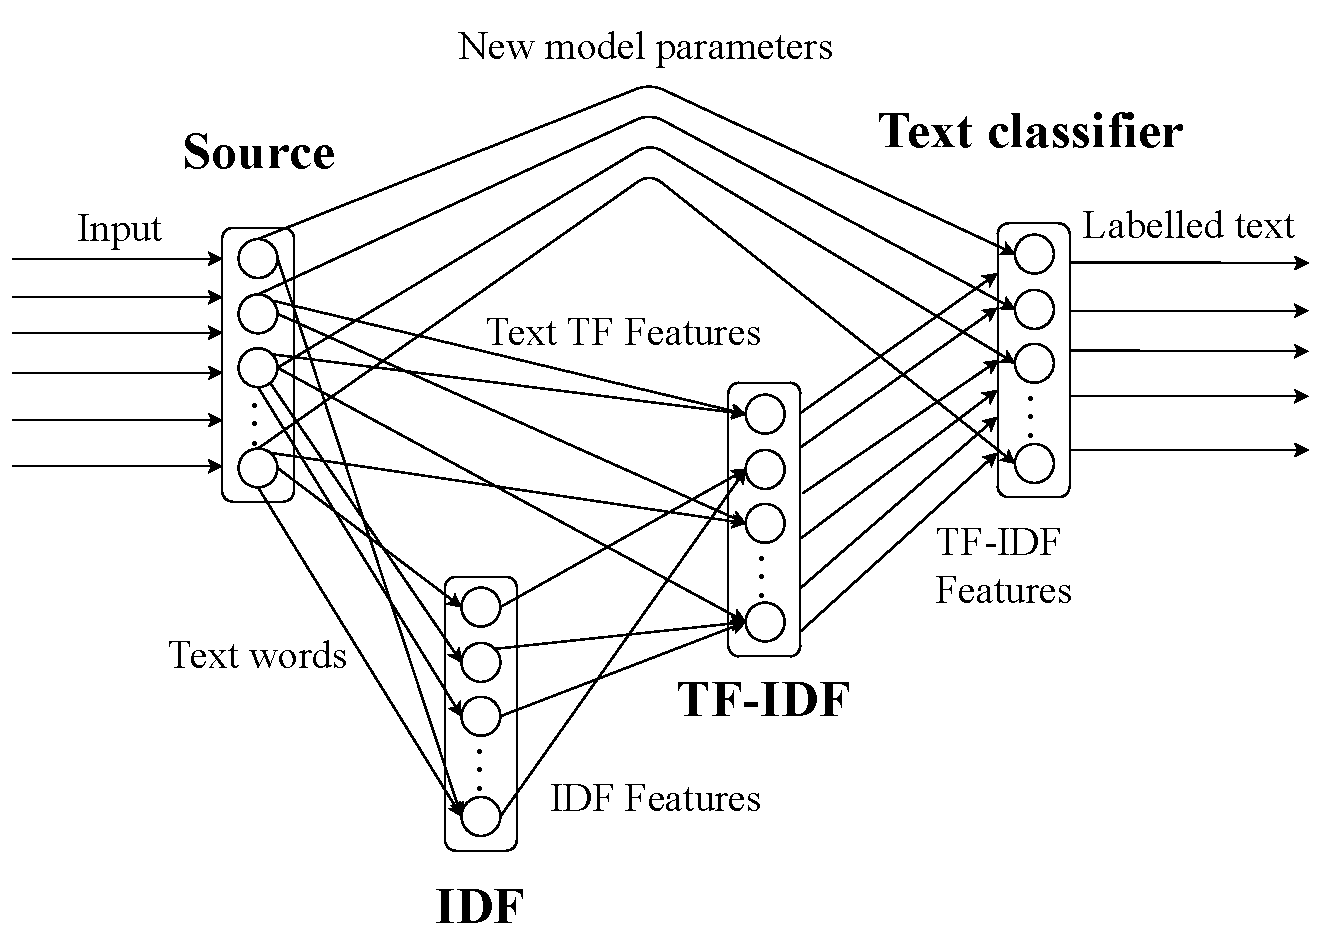
\includegraphics[scale=0.375]{pics/physical-graph}
  \caption{The physical graph}
  \label {physical_graph}
\end{figure}

In~\FlameStream\, all operations from a logical graph are executed on all computational units. Scalability is achieved due to data partitioning before each operation. Figure ~\ref{physical_graph} captures the scheme of a physical execution for the proposed logical graph. Each vertex on the scheme denotes the same computational cluster consisted of multiple units. Data partitioning before {\em IDF} and {\em TF-IDF} operations is defined by keys. Data elements with the same keys are processed on a single computational unit. For {\em IDF} operation the key is a word, while {\em TF-IDF} aggregates items with the same text identifier. As we can see on the scheme, all operations that take part in predicting pipeline scales among all computational units. 

\subsubsection{Training pipeline}

Training pipeline is a special branch within the logical graph introduced above. If a text is already labeled, their features are sent to a {\em Partial fit} vertex instead of the {\em Classifier}. {\em Partial fit} vertex buffers all input elements until training is triggered. It is done using a special input stream element, which is submitted directly to the {\em Input} . Every vertex except the {\em Partial fit} passes this element through without processing. This behavior is similar to punctuations handling~\cite{tucker2003exploiting}. After training, the buffer is flushed. Updated parameters of a machine learning model are saved for further training and broadcasted to all {\em Text Classifier} vertices.

\subsubsection{Dealing with concept drift}

Concept drift refers to the particular meaning of words, which changes over time. This aspect may affect the quality of a prediction, especially for data from news and social media sources. To handle this trait, we compute inverse document frequencies within a sliding window of a user-defined length. Similar approach demonstrates its effectiveness in~\cite{klinkenberg2000detecting}.

\subsection{Machine learning model \label{ML}}

The classifier's model can be chosen independently from other computations. In our case, we use Multinomial Logistic Regression. At the start of the system, the initial classifier parameters such as weights can be provided by a pre-train process.

Every time, when the Partial Fit is triggered, the following process occurs, which can be described in terms of the optimization of a cost function. This function in our case is written below:

\begin{center}

$$ J(W) = -\frac{1}{m} \sum \limits_{i = 1}^{m} \sum \limits_{j = 1}^{k} \mathbbm{1}_{\left\{y^{(i)} == j\right\}} \cdot \log \frac{\exp\left({W_{j}^Tx^{(i)}}\right) }{\sum \limits_{l = 1}^{k}  \exp\left({W_{l}^Tx^{(i)}}\right) }$$ 
 $$ +  \lambda_1 ||W||_1 + \lambda_2 ||W - W_{prev}||_2 $$

\end{center} 

The number of points in a new dataset is denoted as $m$. The point with index $i$ showed as $x^{(i)}$. The number of classes is $k$. New weights are designated as $W$. The weights, that computed in the previous step, are $W_{prev}$. At the first time of triggering the process, $W_{prev}$ are the pre-trained weights. 

The formula provides the goal of the training. The first component is the standard softmax function for multiple classes. The second component keeps the l1 regularization of the weights. The important aspect is the regularization provides sparsity, hence, the model has a small size -- about 1 Mb, which can be stored and updated with low cost. To use the previous history of the classifier weights we apply l2 regularization as the third component. Fitting new points and the consideration of the previous weights ensure better accuracy of the classifier.

We are interested in finding such $W$ that minimizes $J(W)$. Taking derivatives, one can show that the gradient for each class component is:

\begin{center}

$$ \nabla_{W_j} \; J(W) = -\frac{1}{m} \sum \limits_{i = 1}^{m} \left[ x^{(i)} \left( \mathbbm{1}_{\left\{y^{(i)} == j\right\} } - \frac{\exp\left({W_{j}^Tx^{(i)}}\right)}{\sum \limits_{l = 1}^{k}  \exp\left({W_{l}^Tx^{(i)}}\right)} \right) \right] $$
$$ - \; \lambda_1 sign\left(W\right) - \frac{\lambda_2}{2} \left(W - W_{prev} \right), \; j = [1..k] $$

\end{center} 

We use Stochastic Gradient Descent for optimization. In experiments ~\ref{fs-short-experiments} section, model performance is presented.